%---------------------------------------------------------------------------------------%
%					section																%
%---------------------------------------------------------------------------------------%
%\section{Introduction}

The goal of the plugin mechanism is to specify the behavior of a dynamical system and relations. Users can use their own computation methods without re-compile the platform.

%---------------------------------------------------------------------------------------%
%					section																%
%---------------------------------------------------------------------------------------%

Plugin is a set of C functions, but compiled with a C++ compiler (\textit{extern "C"} before the header of the function). It must be supplied as a dynamical library, to allow the platform to load it and use its functions.

Parameters and returned values of function of plugins must be C types (no C++ objects or STL containers). \\

For Integrators which use a FORTRAN routine and pass it a plugin function in parameters, a specific method in the integrator class to make the conversions between C and FORTRAN types (use g2f.h features). \\

From platform point of view, plugin functions are pluged on functions pointers (same signature as the plugin function). A plugin function can be used only if it respects strictly a signature of a pointer function supplied by the platform.

%---------------	sub-section		----------------------------------------------------%
\subsection{Dynamical systems plugins}

\subsubsection{class DynamicalSystem}
\begin{verbatim}
void VectorField(int* sizeOfX, double* time, double* xPtr, double* xdotPtr);
void computeJacobianX(int* sizeOfX, double* time, double* xPtr, double* jacobianXPtr);	
\end{verbatim}

\subsubsection{Class LinearSystemDS}
\begin{verbatim}
void computeF(int* sizeOfF, double* fPtr, double* time);	
void computeU(int* sizeOfU, double* uPtr, double* time);
\end{verbatim}

\subsubsection{Class LagrangianNLDS}
\begin{verbatim} 
void computeMass(int* sizeOfq, double* time, double* qPtr, double* massPtr);	
void computeFInt(int* sizeOfq, double* time, double* qPtr, double* velocityPtr,
double* fIntPtr);
void computeFExt(int* sizeOfq, double* time, double* qPtr, double* fExtPtr);
void computeQNLInertia(int* sizeOfq, double* qPtr, double* velocityPtr,
double* QNLInertiaPtr);	
void computeJacobianQFInt(int* sizeOfq, double* time, double* qPtr, double* velocityPtr, 
double* jacobPtr);
void computeJacobianVelocityFInt(int* sizeOfq, double* time, double* qPtr, 
double* velocityPtr, double* jacobPtr);
void computeJacobianQQNLInertia(int* sizeOfq, double* qPtr, double* velocityPtr, 
double* jacobPtr);
void computeJacobianVelocityQNLInertia(int* sizeOfq, double* qPtr, double* velocityPtr, 
double* jacobPtr);
\end{verbatim}

%---------------	sub-section		----------------------------------------------------%
\subsection{Relations plugins}

\subsubsection{Class Relation}
\begin{verbatim}
void computeOutput(double* xPtr, double* time, double* lambdaPtr, double* yPtr);
void computeInput(double* xPtr, double* time, double* lambdaPtr, double* rPtr);
\end{verbatim}

\subsubsection{Class LagrangianNonLinearR}
\begin{verbatim}
void computeJacobian(int* sizeOfQ, double* qPtr, int* sizeOfY, double* jacobPtr);	
void computeH(int* sizeOfQ, double* qPtr, int* sizeOfY, double* yPtr);
\end{verbatim}

%---------------	sub-section		----------------------------------------------------%
\subsection{Matrices representation}

Platform and plugin functions are coded in C/C++, but double pointers representing vectors and matrices given in parameters are column-oriented (FORTRAN format), in order to be used simply with FORTRAN computation libraries, e.g. Blas. \\

This is an example : \\

\[M=\left(
\begin{array}{cccc}
1 & 2 & 3 & 4 \\
5 & 6 & 7 & 8 \\
9 & 10 & 11 & 12 \\
\end{array}
\right)\]

n = 3 and m = 4 (indices start at 0 in C language). \\

MFor is the array in memory representing M. Its elements are sorted as follows :

\begin{tabular}[h]{|c|c|c|c|c|c|c|c|c|c|c|c|}
\hline
%\multicolumn{3}{|c|}
1 & 5 & 9 & 2 & 6 & 10 & 3 & 7 & 11 & 4 & 8 & 12 \\
\hline 
\end{tabular} \\

To access to element Mij of matrix M, we need to compute its position in the array : MFor[i + jn].
For example, this is a short C function which returns a M element form its coordinates in the matrix :

\begin{verbatim}
int getMatrixElement(int i, int j, int n, int m, int MFor[])
{
        // i and j are the coordinates of the element in the matrix M
        // n is the number of lines of M
        // m is the number of columns of M
        // MFor is the array representing the matrix M
	
        return MFor[i + j * n];	
}
\end{verbatim}

If we try to get the element $M_{1,3}$ :
\begin{verbatim}
printf("searched element is : \%d", getMatrixElement(1, 3, 3, 4, MFor));
\end{verbatim}

The result displayed on the screen is : \textsf{searched element is : 8}.\\

%---------------------------------------------------------------------------------------%
%					section																%
%---------------------------------------------------------------------------------------%
\section{"False"plugin}
False plugin system allows an integrateur dedicated to a dynamical systems class to integrate its derivated classes too. For example :

\begin{itemize}

\item class DynamicalSystem \\
system : 
\begin{displaymath} \dot x = f(x, t) \end{displaymath} 
\begin{displaymath} \nabla_x f(x, t) \end{displaymath} 


f is a plugin function and is plugged to vectorField function pointer to the platform.
$ \nabla_x f$ is a plugin function and is plugged to computeJacobianX function pointer to the platform. \\

\item  Integrator I, dedicated to integration of systems represented by Dynamicalsystem class.  

\item Class LinearDS, specializes DynamicalSystem class. \\
syst�m :
\begin{displaymath} \dot x = Ax \end{displaymath} 
\begin{displaymath} \nabla_x f(x, t) \end{displaymath} 

\begin{displaymath} f(x, t) = Ax \end{displaymath} 
\begin{displaymath} \nabla_x f(x, t) = A \end{displaymath} 

Functions f and $\nabla_x f $ are in this case very simple and directly supplied by internal methods of LinearDS class. These methods are plugged to the platform during the initialisation phase instead of plugin functions.

\end{itemize}

During the integration, integrator I dedicated to DynamicalSystem class calls f et $\nabla_x f $ functions during computation. It can therefore integrate a LinerDS object since required functions are supplied by the class and respect plugin functions signatures.

In a general manner, every class derivated from another which uses plugin system must use plugin functions too, or supply internal functions which can be plugged instead.

%\begin{ndr} 
%Ajouter un sch�ma ? \\
%\end{ndr}

\begin{figure}[h]
\begin{center}
\includegraphics[scale=0.40]{figure/Plugin.ps}
\caption{General diagram of false plugin mechanism}
\label{fig: General diagram of false plugin mechanism}
\end{center}
\end{figure}


%---------------------------------------------------------------------------------------%
%					section																%
%---------------------------------------------------------------------------------------%
\section{\acs{lmgc90} plugin}
\subsection{Integration into the \acs{kernel}}
This plugin is designed to give specific data required by \acs{kernel} to make a simulation with complex contact detection.
It makes low level computations for the \acs{kernel} to be able to do simulation steps.

\subsection{Data communications}
Data transmission is bidirectionnal between \acs{kernel} and \acs{lmgc90} plugin.\\
The \acs{kernel} needs modeling data supplied by the plugin in modeling phase. Moreover the plugin gives data at the beginning of each steps of the simulation to for the \acs{kernel} to have the good data to make simulation computations.\\
In the other way, the plugin receive informations at the end of each time step as an update of the state of the system.

\subsection{Data to send}
\begin{itemize}
	\item Data loading from \acs{lmgc90} model, to the \acs{kernel} :\\
	number of dynamical systems\\
	q and q dot for each dynamical system\\
	M matrix\\
	Fext at each step\\
	blocking constraints\\
	
	\item Update of the \acs{lmgc90} model :\\
	q and q dot\\
	reaction forces\\
\end{itemize}

%---------------------------------------------------------------------------------------%
%					section																%
%---------------------------------------------------------------------------------------%
\section{Example of a plugin development}

%---------------	sub-section		----------------------------------------------------%
\subsection{Header file}

\textbf{This file is not compulsory in C.}

This is a template of plugin header file, named \textit{plugin\_example.h}:

\begin{verbatim}
#ifndef _PLUGIN_EXAMPLE_
#define _PLUGIN_EXAMPLE_

// decalration of functions of the plugin
extern "C" 
{
	void function1(...);
	...
	void functionN(...);	 
}
#endif //_PLUGIN_EXAMPLE_
\end{verbatim}

%---------------	sub-section		----------------------------------------------------%
\subsection{Source file}

This is the plugin source file, named \textit{plugin\_example.C}:

\begin{verbatim}
#include "plugin_example.h" // if it exists
#include ...

// impl�mentation of plugin functions
extern "C"
{ 
        void function1(...)
        {
                ...
        }

        ...

        void functionN(...)
        {
                ...	 
        }
}
\end{verbatim}

%---------------	sub-section		----------------------------------------------------%
\subsection{Compilation and creation of the dynamic library.}

To build the plugin under Linux (or UNIX), follow the instructions : \\

First, the C file have to be built :
\begin{verbatim}
g++ -g -fbounds-check -w -Wno-deprecated -fPIC -c plugin_example.C
\end{verbatim}

This operation creates a file plugin\_example.o if there are no compilation errors.

\begin{verbatim}
g++ -g -fbounds-check -w -Wno-deprecated -fPIC -shared -W -O plugin_example.C 
-o plugin_example.so
\end{verbatim}

This operation creates the dynamical library plugin\_example.so. Plug-in is ready to use.

%---------------	sub-section		----------------------------------------------------%
\subsection{Plugin and XML file.}

%\begin{ndr} 
%un paragraphe sur le mode de branchement des plugin via le XML ?
%\end{ndr}

Let's take an example. we imagine "function1" of our previous plugin example is used for computing the mass matrix of a non linear Lagrangian system (LagrangianNLDS class of the platform) : we have to indicate to the platform that for the system we want to simulate, computing mass function which is used is function1 of the plugin plugin\_example.
(for more explanations about XML Input data, you can read \ac{sum}) \\

\begin{verbatim}
<DS number='1' type="LagrangianNLDS">
        <Id> DS1 </Id>
        ...	
        <M matrixPlugin="plugin_example:function1"/>
        ...
</DS>
\end{verbatim}


The platform can load the plugin\_example library during the execution only if it knows the path of the plugin on the computer. There are two cases :

\begin{itemize}

\item plugin\_example library.so is in the same repertory as platform exe file : it should work directly.

\item plugin\_example library.so is not in the same repertory as platform exe file : its access path must be added in environment variable LB\_LIBRARY\_PATH. Platform will seek the plugin in this specified path. This is an example of command line to set LB\_LIBRARY\_PATH :



\begin{verbatim}
setenv LD_LIBRARY_PATH /your_path/plugin_example/:$LD_LIBRARY_PATH
\end{verbatim}
\end{itemize}

